\section{Lattice Boltzmann simulation}
\tododone[inline]{Christie}{LBM done}
\todointern[inline]{Christie}{Someone proofread}
In order to numerically simulate fluid (for eg: the river in "Grand Theft Boat - Sarntal") we used the well known Lattice Boltzmann method. The choice
of this method can be attributed to its simplicity.The code we implemented was based on a D2Q9 stencil, i.e a 2D grid with 9 Probability Distribution Functions (PDFs) per cell (See Figure \ref{fig: D2Q9 push scheme}). 

	
\begin{figure} [h]
\centering
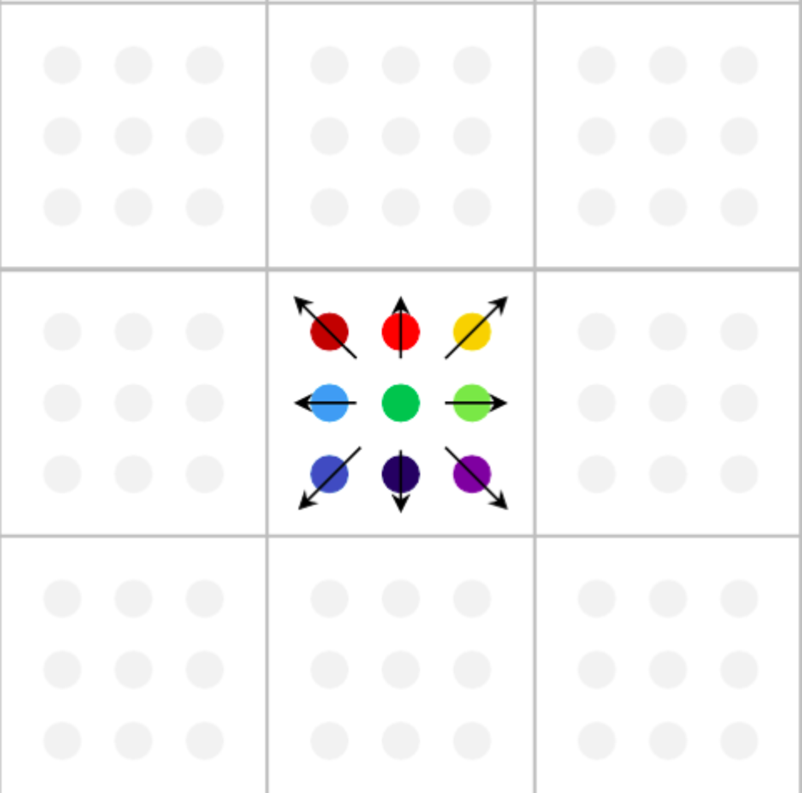
\includegraphics[scale=0.4]{img/LBM/D2Q9_push}
\caption{LBM - D2Q9}
\label{fig: D2Q9 push scheme}
\end{figure}

\subsection{LBM Algorithm} \label{sec:LBM_algorithm}
	The Lattice Boltzmann algorithm is, structurally, an explicit time stepping method. Each of the time steps consists of
	\begin{itemize}
		\item update call type and initialise new cells
		
		\item calculation of the local equilibrium distributions
		$f^{\mathrm{eq}}$ using the refreshed macroscopic density and velocity
		\item weighing between equilibrium distribution and density
		distribution functions from the previous time step
		to model particle interactions
		\begin{equation}
		\label{eq:LBMalgorithm1}
		f_i^*(x , t + \delta t) = f_i(x, t)
		- \omega [f_i(x, t) - f_i^{\mathrm{eq}}(\rho, u)]
		\end{equation}

		%relaxation towards equilibrium step. Mass and momentum preservation.
		\item streaming of PDFs depending on their movement direction
		\begin{equation}
		\label{eq:LBMalgorithm2}
		f_i(x + c_i \delta t,\, t + \delta t) = f_i^*(x , t + \delta t)
		\end{equation}

		\item boundary treatment
	\end{itemize}
	
	\begin{figure}[ht]
		\centering
		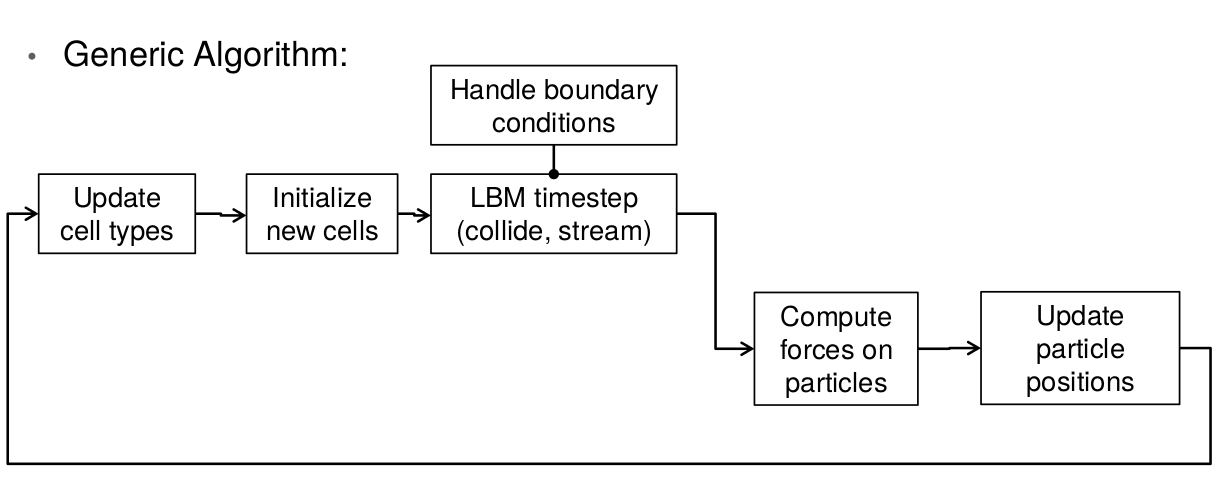
\includegraphics[scale=0.25]{img/LBM/generic_algorithm.png}
		\caption{Generic Algorithm of LBM}
		\label{fig: LBMGeneric_algorithm}
	\end{figure} 
	
\subsection{Implementation}
The LBM stage kicks in once it receives the flag fields (called \texttt{levelGeometry} internally in LBM code) and information about rigid bodies in the form of iterators through the interface between $RigidBodies$ and $LBM$ (RigidBodyInterface). Then one timestep of LBM simulation is 
carried out (as described below). Finally, the velocities of fluid along with
the force acting on rigid bodies are sent out as output. The basic framework of
LBM is shown as UML diagram in figure \ref{fig: LBMUMLgraph}. It is worthy to note that the 
definition of some functions in \texttt{CStage_Fluid_SimulationLBM} could be found in \texttt{LBMSimulation.cpp}(this was due to the last minute change in the structure of the code).
\begin{figure}[ht]
	\centering
	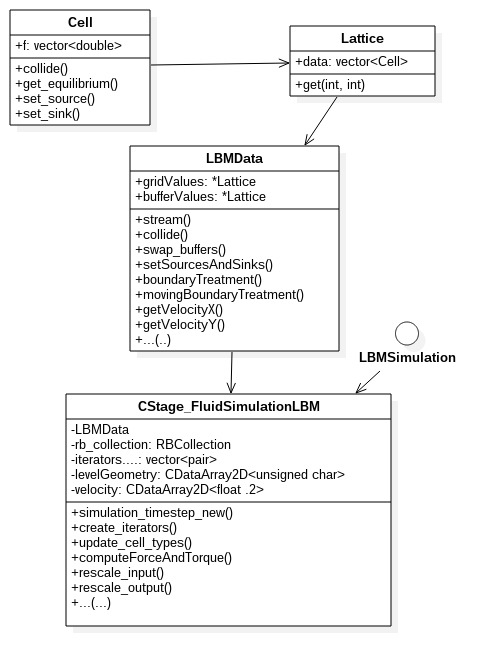
\includegraphics[scale=0.5]{img/LBM/LBM_uml.jpg}
	\caption{UML diagram of LBM}
	\label{fig: LBMUMLgraph}
\end{figure} 
\subsection *{Update cell Types}
Since our simulation needs to be dynamic; i.e the rigid body(RB) objects move during
the simulation, one has to continuously adapt the flag fields during the course of simulation. This is realized by, first, reinitializing all the \texttt {cell_type_rigid_body} flags to fluid and then initializing the \texttt{cell_type_rigid_body} to the current RB objects, from the positional data
received through the RigidBodyInterface. Such implementation could be found in \texttt{CStageFluidSimulation::update_cell_types}. Additionally, one needs to initialize the newly uncovered cells. A common approach is to interpolate the density from surrounding cells and velocity of next particle point, but here in our implementation we simply set them to equilibrium.
\subsection *{Stream}
 In the streaming step, we just need to push data at the current cell to the neighboring cells in the respective direction (we implemented a push scheme). In order not
 to overwrite the current data, we had two arrays to hold the current and the 
 modified data, which we swap after each time step. The streaming step is implemented under the \texttt{LBMData} class. 
 
 \subsection *{Collision} \label{subsection:collision}
 The collision is a local operation to each cell  which requires solving equation \ref{eq:LBMalgorithm1} presented in LBM Algorithm section [\ref{sec:LBM_algorithm}].The computation of macroscopic density and velocity needed to calculate equilibrium are carried out using:
 \[\rho_j = \sum_{\mathrm{PDFs}} f_i\qquad u_j = \frac{1}{\rho_j} \sum_\mathrm{PDFs}
 c_i\]
 
  Implementation of collision operator can be seen under the \texttt{Cell} class.
 
 
 Although we had initially a fused stream collide version of the LBM (for performance reasons), but then we had a major structure reordering in the last version, for reasons of readability of the code and to assist debugging, which employs separate kernels for stream(push-scheme) and collide.
 
\subsection *{Boundary Treatment}
This is a crucial step in an LBM simulation and one which defines the interaction
between other groups. Basically, we had two kinds of boundaries; no-slip boundaries and moving boundaries. 
\subsubsection *{No-slip boundary}
  Basic no-slip boundaries were used for some non-moving obstacles and the domain boundaries. Here the PDFs just bounces back, (i.e PDF direction is flipped) on the boundary this signifies that the velocity is basically 0 at the boundary. The implementation could be found under \texttt{LBMData::boundaryTreatment()}.


\subsubsection *{Moving No-slip boundary}
Furthermore, we implemented boundaries for moving rigid body obstacles(eg: boats). This was the key to the one-side of coupling, namely Rigid-body to Fluid. 
\begin{figure}[ht]
	\centering
	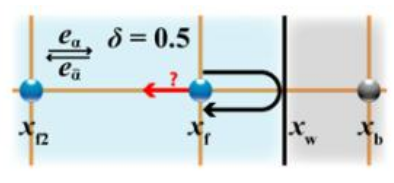
\includegraphics[scale=0.5]{img/LBM/moving_boundary.png}
	\caption{Moving boundary treatment}
	\label{fig: Moving boundary}
\end{figure} 
 The implementation is similar to no-slip, however, it also takes the velocity of the moving object into account. Figure \ref{fig: Moving boundary} along with equation [\ref{eq:LBMalgorithm3}] illustrate the procedure. 

	 \begin{equation}
	 \label{eq:LBMalgorithm3}
	f_{\bar{\alpha}}(x_f , t + \delta t) = (1+\delta)^{-1} f_\alpha(\boldsymbol{x_f}, t+\delta t)
	+ \delta.f_\alpha(\boldsymbol{x_b}, t+\delta t) + \delta . f_{\bar{\alpha}}(\boldsymbol{x_{f2}}, t+\delta t) - 6c^{-2}[\omega_{\alpha}\rho_w \boldsymbol{e_a.u_w}]
	\end{equation}


Where:\\
\hspace*{3em}
\begin{tabular}{rl}
	$f\i$:& are the PDFs in the corresponding directions as shown in figure \ref{fig: Moving boundary}  \\
	$x\i$ :& are the grid points considered \\
    $\omega_{\alpha}$:& the standard weights \\
\end{tabular}

If we set the velocity to 0 we get back to the no-slip condition. The same formula is used in \texttt{LBMData::movingboundaryTreatment} to realize the
moving boundary condition. The wall velocity $u_w$ and the wall distance $\delta$ 
are obtained from the rigid body object.

\subsection *{Compute Force and Torque}
In order to make the simulation more realisitic, one needs to take into account also the force exerted by the fluid on rigid body i.e Fluid - Rigid Body interaction. We realized this using a momentum exchange method; i.e we just compute the momentum (as explained in collision step for calculating velocity [\ref{subsection:collision}]) at particle-fluid node pairs to get the force.
%\begin{equation}
%F = \sum_b \sum_{i=1}^8 c_i*(f_i(x_b,t)+f_{i^-(x_f,t)})*\delta x/\delta t
%\end{equation}
Once we obtain the force on a body, we then calculate the force and the corresponding torque, with the help of center of mass of the body (input from RigidBodyInterface). The computed force and torque are then sent through the RigidBodyInterface for further processing.
The implementation of this could be found under \texttt{CStage_FluidSimulationLBM::computeForceAndTorque()}

\subsection{Domain scaling}
Since LBM solver is a quite expensive and memory bound algorithm, it turned out that
we had difficulties in carrying out the simulation in real-time for bigger domains, as required by "Grand Theft Boat - Sarntal". To keep up with the game's frame rate, we scaled down our domain internally; where the simulation was carried out and then interpolated our output velocity before sending it to further processing. This can be seen in \texttt{CStage_Fluid..LBM::rescale_input()} and \texttt{rescale_output()}



%	\item LBM code framework structure
%	The LBM stage receives the flag fields (called levelGeometry internally in LBM code) in the form of iterators from the Rigid Body group. 
%	\item Fluid to Rigid Body interaction
%	\item Rigid Body to fluid interaction
%	\item How to build it
